
\subsection{exercise 0}
\begin{enumerate}
    \item $g(x) = \lambda_2\|x\|_1$ then $\prox_g(x)= \mathcal{T}_{\frac{\lambda_2}{L_f}}(x)$
    \item $g(x) = \frac{\lambda_1}{2}\|x\|^2_2 + \lambda_2\|x\|_1$ then $\prox_g(x)= \mathcal{T}_{\frac{\lambda_2}{L_f+\lambda_1}}(\frac{x}{\frac{\lambda_1}{L_f}+1})$
    \item the code is \emph{ex-p2-e0.py}
    \item V-FISTA 1, i.e. on $g(x) = \lambda_2 \|x\|_1$, performs the best
    \item $x^{sol}_{PGM}(1:4)=(-0.4397, 0.0197, 1.4228, -0.8781)$\\
     $x^{sol}_{FISTA}(1:4)=(-0.4320, 0.0288, 1.4337, -0.9066)$\\
     $x^{sol}_{V-FISTA 1}(1:4)=(-0.43210748, 0.02959795, 1.43437278, -0.90583604)$\\
     $x^{sol}_{V-FISTA 2}(1:4)=(-0.43210796, 0.02959784, 1.43437041, -0.90583332)$
    \begin{figure}[h]
        \centering
        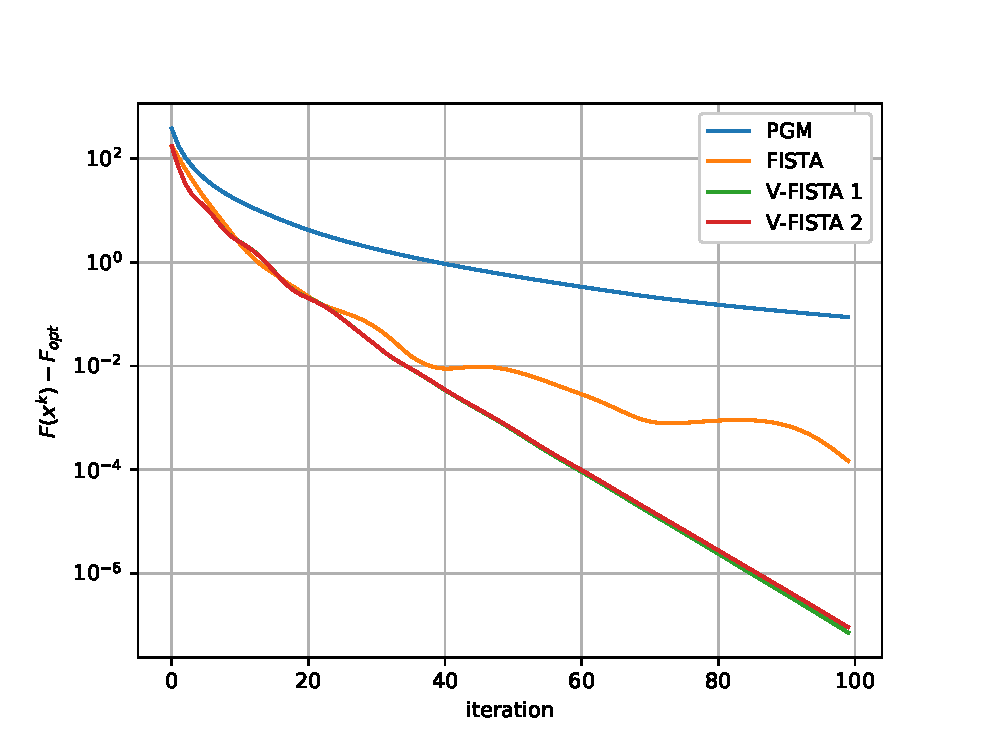
\includegraphics[scale=0.5]{codes/result_images/ex_p2_e0_results.eps}
        \caption{Part 2, exercise 0, V-FISTA 1 is with $g=\lambda_2\|\cdot\|_1$, and V-FISTA 2 is with $g=\frac{\lambda_1}{2} \|\cdot\|^2_2 + \lambda_2\|\cdot\|_1$}
        \label{fig:p2e0}
    \end{figure}
\end{enumerate}




\subsection{exercise 1}
\begin{enumerate}
    \item $H(\bm x) := \bm x^T \bm Q \bm x + 2 \bm b^T \bm x + c$ \\
    $\nabla H(\bm x) = 2 \bm b + 2 \bm Q \bm x = 0$, then $\bar{\bm x} = - \bm Q^{-1} \bm b$ \\
    $H(\bar{\bm x})=\bm b^T \bm Q^{-T} \bm Q \bm Q^{-1} \bm b - 2 \bm b^T \bm Q^{-1} \bm b + c \geq 0$ \\
    $\Rightarrow c \geq \bm b^T \bm Q^{-1} \bm b$

    \item as $Q$ is positive definite, one can decompose it to have\\
    $f(\bm x) = \sqrt{\bm x^T \bm Q \bm x + 2 \bm b^T \bm x + c} = \sqrt{\|Px - v\|_2^2+ c'^2} = \|\begin{pmatrix}
        Px-v \\
        c'
    \end{pmatrix}\|_2$\\
    where if $Q=U\Lambda U^T$, $P:=\Lambda^{\frac{1}{2}}U^T$, $v:=-\Lambda^{\frac{-1}{2}}U^Tb$, and $c'^2:=c-b^T Q^{-1} b$. As $\ell_p$ norm with $p \geq 1$ is convex, and composition of a convex function with an affine mapping is also convex, this norm is convex. Also sum of two convex function is convex, hence, the problem is convex.
    
    \item $f(\bm x) = \sqrt{\bm x^T \bm Q \bm x + 2 \bm b^T \bm x + c}, \quad g(\bm x) = 0.2 \|\bm D \bm x\|_1$\\
    $\nabla f(\bm x) = \frac{2 \bm b + 2 \bm Q \bm x}{2 \sqrt{H(\bm x)}}$\\
    $\prox_{\frac{0.2}{L_f} \|\cdot\|_1}(\bm x) = \mathcal{T}_{\frac{0.2}{L_f}}(\bm x)$
    \begin{align*}
        \prox_{\frac{g}{Lf}}(\bm x) &= \prox_{\frac{0.2}{L_f}\|\cdot\|_1 \circ \bm D}(\bm x) = \bm x + \bm D^T \prox_{\frac{0.2}{L_f} \|\cdot\|_1}(\bm D \bm x) - \bm D \bm x \\
        & = \prox_{\frac{0.2}{L_f} \|\cdot\|_1 \circ \bm D}(\bm x) = \bm x + \bm D^T \mathcal{T}_{\frac{0.2}{L_f}}(\bm D \bm x) - \bm D \bm x\\
    \end{align*}

    \item to estimate $L_f$ we upper bound the Hessian of the function $f$. We have:\\
    $\nabla^2 f(x) = \frac{1}{\sqrt{\|Px-v\|^2 + c'^2}}P^T \left[I - \frac{(Px+b)(Px+b)^T}{\|Px-v\|^2 + c'^2}\right]P$\\
    the eigenvalues of the bracket belong to $\{0,1\}$, as the matrix inside is a product of one vector by itself. We upper bound the Hessian as:
    $\nabla^2 f(x) \leq \frac{\|P\|^2}{\sqrt{\|Px-v\|^2 + c'^2}} \leq \frac{\|P\|^2}{c'}$, Hence,\\
    $L_f = \frac{\|\Lambda\|}{\sqrt{c-b^T Q^{-1} b}}=\frac{\|Q\|}{\sqrt{c-b^T Q^{-1} b}}$

    \begin{figure}[h]
        \centering
        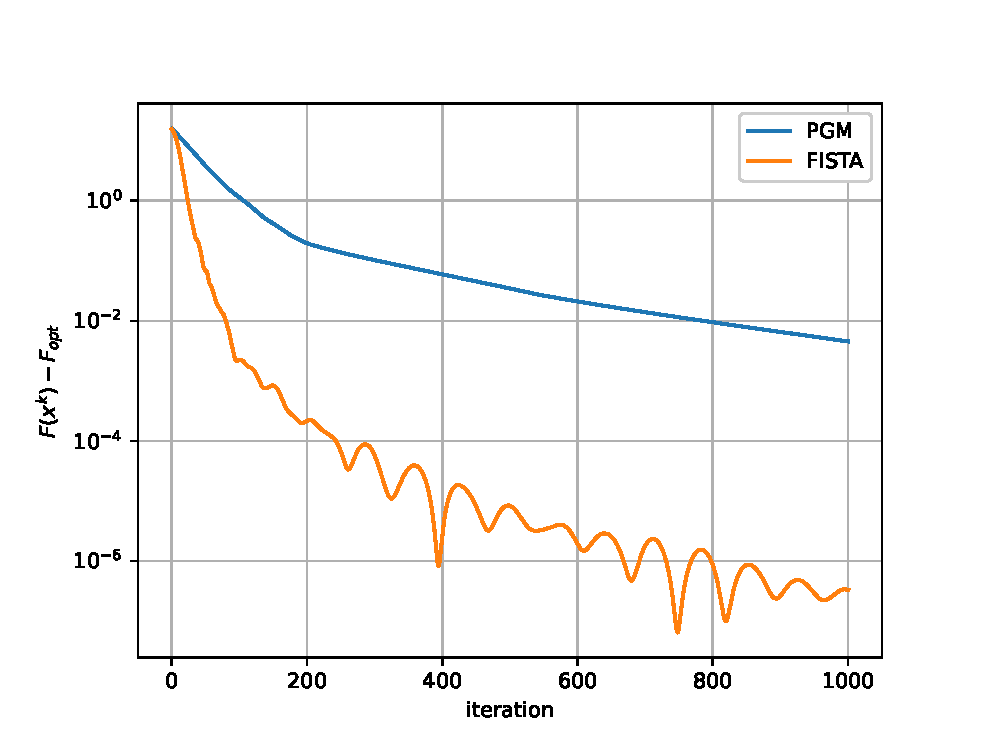
\includegraphics[scale=0.5]{codes/result_images/ex_p2_e1_results.eps}
        \caption{Part 2, exercise 1}
        \label{fig:p2e1}
    \end{figure}

    \item the stepsize used in PGM is $\gamma = \frac{1}{L_f}=0.02027373$

    \item iterates:\\
    PGM:\\
    $iter\;1:\; F(x^k)-F_{opt}: 15.969037688894332\\
    iter\;101:\; F(x^k)-F_{opt}: 1.138840371899061\\
    iter\;201:\; F(x^k)-F_{opt}: 0.19536585866318035\\
    iter\;301:\; F(x^k)-F_{opt}: 0.10256671457047162\\
    iter\;401:\; F(x^k)-F_{opt}: 0.05981160382616579\\
    iter\;501:\; F(x^k)-F_{opt}: 0.034541962530351356\\
    iter\;601:\; F(x^k)-F_{opt}: 0.021032280748006116\\
    iter\;701:\; F(x^k)-F_{opt}: 0.013937040643956067\\
    iter\;801:\; F(x^k)-F_{opt}: 0.009469387714531763\\
    iter\;901:\; F(x^k)-F_{opt}: 0.0065280945179999605\\
    iter\;1001:\; F(x^k)-F_{opt}: 0.004544681858035915\\$

    FISTA:\\
    $iter\;1:\; F(x^k)-F_{opt}: 15.616787710263878\\
    iter\;101:\; F(x^k)-F_{opt}: 0.002229198785176578\\
    iter\;201:\; F(x^k)-F_{opt}: 0.00021635498722005764\\
    iter\;301:\; F(x^k)-F_{opt}: 5.744173655841678e-05\\
    iter\;401:\; F(x^k)-F_{opt}: 2.7570780005703455e-06\\
    iter\;501:\; F(x^k)-F_{opt}: 8.335118572233569e-06\\
    iter\;601:\; F(x^k)-F_{opt}: 1.9008889147187347e-06\\
    iter\;701:\; F(x^k)-F_{opt}: 1.7973270658444562e-06\\
    iter\;801:\; F(x^k)-F_{opt}: 8.541816285401183e-07\\
    iter\;901:\; F(x^k)-F_{opt}: 2.646209011913925e-07\\
    iter\;1001:\; F(x^k)-F_{opt}: 3.302678983629903e-07$\\

    \item solutions:\\\\
    PGM: $(-0.17302056, -0.13170504,  0.2853231 , -0.26288016, -0.53923318,\\ -0.41890723,  0.34400762, -0.51913402,  0.38304034, -0.8028364 , \\-0.156584  , -0.27559503,  0.06735174, -0.17116589, -0.07071933,\\ -0.07055706, -0.0558151 , -0.13077329, -0.10362827,  0.16621555,\\ -0.74600957, -0.41574597, 0.62302217, -0.33120591, -0.24841553,\\ -0.63743909, -0.34855206,  0.2553829 , -0.13449554, -0.0940163 )$\\\\
    
    FISTA: $(-0.23010618, -0.13942272,  0.31427133, -0.27633859, -0.59820196,\\       -0.49575369,  0.34118456, -0.5456482 ,  0.38702184, -0.91169326,\\       -0.17665491, -0.32830946,  0.02846801, -0.10373275, -0.14537967,\\       -0.07446206, -0.03326546, -0.1831482 , -0.08021404,  0.26755059,\\       -0.84049738, -0.48603082,  0.65971966, -0.25551334, -0.2822796 ,\\       -0.75444863, -0.35508949,  0.28620091, -0.20633458, -0.18046632)$

\end{enumerate}


\subsection{exercise 3}
\begin{enumerate}
    \item $f(x)=\frac{1}{2}\|x\|_2^2$, and it is strongly convex with $\sigma=1$
    \item $g(A x) := C \sum_{i=1}^n{\max\{0,1-y_i \bm w^T \bm x_i\}}$, take $C=1$\\
    $A = \diag(\bm y) \bm X$, where $\bm y=(y_1,\dots,y_n)$ and $\bm X$ has rows equal to $\bm x_i$\\
    $L_f = \|A\|^2/\sigma$\\
    $g(z) = h(1-z)$ where we define:\\
    $h(z) := \sum_{i=1}^n \{0, z_i\} = \sigma_{\boxx[0,1]}(z)$\\
    $\prox_{L_f h}(x)=z-L_f P_{\boxx[0,1]}(\frac{x}{L_f})$\\
    $\prox_{L_f g}(x) = 1 - \prox_{L_f h}(1 - x) = x + L_f P_{\boxx[0,1]}(\frac{1-x}{L_f})$

    \item DPG iterates:\\\\
    $x^k = A^T y^k$\\
    $y^{k+1}=y^k - \frac{1}{L_f}A x^k + \frac{A x^k - L_f y^k}{L_f} + P_{\boxx[0,1]}(\frac{1-A x^k + L_f y^k}{L_f})$

    \item solutions:\\\\
    by DPG: $(2.04031854, -0.91262279)$\\
    by FDPG: $(2.13382443, -1.01718168)$

    \begin{figure}[h]
        \centering
        \includegraphics[scale=0.5]{codes/result_images/ex_p2_e3_results.eps}
        \caption{Part 2, exercise 3}
        \label{fig:p2e3}
    \end{figure}

    
\end{enumerate}
